% Beijing 2011 tetrahedron schematic: AB/DG/EF dashed, rest solid.
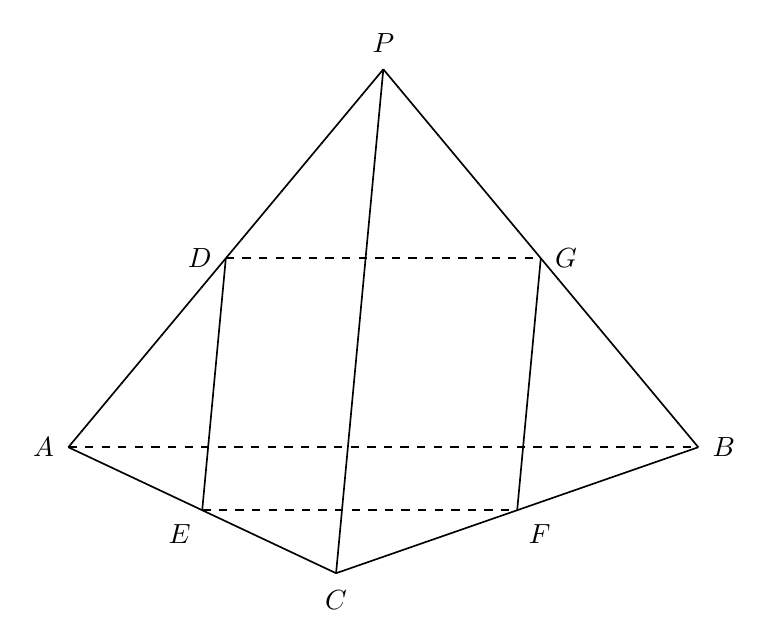
\begin{tikzpicture}[x=1cm,y=1cm,font=\normalsize,
  geometry edge/.style={draw=black,solid,line width=.6pt},
  geometry hidden/.style={draw=black,dashed,line width=.6pt},
  geometry label/.style={font=\normalsize,inner sep=2pt,fill=none}]
\coordinate (P) at (4.0,6.4);
\coordinate (D) at (2.0,4.0);
\coordinate (G) at (6.0,4.0);
\coordinate (A) at (0.0,1.6);
\coordinate (B) at (8.0,1.6);
\coordinate (E) at (1.7,0.8);
\coordinate (F) at (5.7,0.8);
\coordinate (C) at (3.4,0.0);
\draw[geometry hidden] (A)--(B);
\draw[geometry hidden] (D)--(G);
\draw[geometry hidden] (E)--(F);
\draw[geometry edge] (P)--(D)--(A);
\draw[geometry edge] (P)--(G)--(B);
\draw[geometry edge] (P)--(C);
\draw[geometry edge] (A)--(E)--(C);
\draw[geometry edge] (B)--(F)--(C);
\draw[geometry edge] (D)--(E);
\draw[geometry edge] (G)--(F);
\node[geometry label,above,yshift=4pt] at (P) {$P$};
\node[geometry label,left,xshift=-3pt] at (D) {$D$};
\node[geometry label,right,xshift=3pt] at (G) {$G$};
\node[geometry label,left,xshift=-3pt] at (A) {$A$};
\node[geometry label,right,xshift=3pt] at (B) {$B$};
\node[geometry label,below left,xshift=-2pt,yshift=-3pt] at (E) {$E$};
\node[geometry label,below right,xshift=2pt,yshift=-3pt] at (F) {$F$};
\node[geometry label,below,yshift=-4pt] at (C) {$C$};
\end{tikzpicture}